\subsection{Completed current execution and independent checks}
The scientific source, draw and acquired actors remain F, D and M as stated
above. The separately published exact continuation source R is
\nolinkurl{0fe0f2bbf76529201a1890db0fc2a94b0be44418}; the recovery
workflow source S is
\nolinkurl{6ab1f9d4f1f9eb70014a7d104b84a499b64ba84c}.
The actual recovery run is
\href{https://github.com/TrillionniumFoundation/NBO/actions/runs/39691016040}{39691016040}.
Its successful status covers recovery of the frozen science, canonical
independent evaluation, statistics, adapted reporting and their stated
checks. It is not a success declaration for a later author manuscript or
referee-ready package.

The interrupted independent execution had 716 saved evaluations. Their
native witnesses were validated before reuse. Eight subsequent segments
made 151, 63, 67, 75, 42, 68, 73 and 86 fresh evaluations, respectively:
625 additional evaluations and 1,341 represented evaluations in total.
The fixed precision ladder and request order were retained. Planned
checkpoint exits in the first seven segments are preserved as such;
the eighth completed the segment schedule. A zero-new-query canonical
finalizer assembled the complete independent account. There are 865 unique
policy keys and 257,469 terminal witness records. Reuse of an evaluation
is not charged as a newly executed original-model query.

The saved composite verifier makes 1,877,650 checks and the saved core
verifier makes 1,198,329 checks through the report stage. These numbers
identify the actually saved receipts, not a count recovered from an earlier
lost local draft. Check counts alone do not establish mathematical truth.
Their substantive coverage includes the immutable source and primary
identities, cache-chain witnesses, canonical-output equalities, the full
fixed catalogue, algebraic acceptance conditions, independent economics,
simultaneous inference and the corrected timing endpoints. The accepted
claims, confirmed gain bounds and contained candidate intervals each
number 824; unresolved accepted joint checks number zero. Independent
complete-policy intervals use the optimal-future original $q$ with the
proved allowance for the unchanged last-date controller. They are not
presented as an independent replay of every last-date rounded action.

The report's protocol adapter preserves the failed frozen-code report and
its diagnostic price tables. It removes a duplicate equal keyword and
matches each 16-state timing clock to the economics of those same states.
The original erroneous use of the 32-state economic cohort with those
clocks is retained as a diagnostic, with 384 old menus and 28,800 old
constraints. The corrected tables contain all 384 menus, 96 complete
three-clock intersections and 28,800 comparator constraints. Neither
version changes a policy, a sample, a trained actor, an original service
clock or a prespecified competitor.

The required restrictive earlier-clock sensitivity has also actually executed
from the saved evidence at
\nolinkurl{results122/final-clock-sensitivity03}. The complete earlier
process supplies 174 cohorts, 2,784 timed decisions and 7,200 additional
competitor constraints. Intersecting it with the current three-clock menus
leaves all 96 sufficient and optimistic four-clock domains empty. Every
four-clock domain was checked to be a subset of its current three-clock
domain. The partial second earlier process is not treated as a complete
scenario. This calculation performs no retiming, new economic query or
additional population draw.

\subsection{The complete statistical and cost account}
The complete outcome catalogue has 174 policy cells, 116 treatment-versus-
own-control contrasts, 232 threshold-event bounds and 348 signed population
comparisons. It uses exactly 32 independent state units. The primary and
timing records contain 5,568 and 8,352 decisions, respectively; timing
repeats do not increase the independent sample size. The simultaneous
failure allocation remains $1/100$ for safe means, $1/100$ for threshold
events and $3/100$ for signed comparisons, totaling $1/20$.
Positive safe population lower bounds occur in 102 cells. None of the
348 signed intervals is strictly positive or strictly negative.
All negative, zero, unresolved and conventional-winner comparisons remain.

All 808 paid refinement attempts completed, and all 12 qualification
refusals are charged. Zero candidate-action economic queries is a
property of this enhancement after its anchor has been qualified; it is
not zero information cost for the Bellman problem. Complete clocks retain
historical acquisition, fitting, finite-training audits, rejected
candidates, certificate arithmetic, loading, inference and process overhead.
The full research ledger separately records independent validation, report
construction, failures, recovery, source checking and publication.
The reporter's field headed
\nolinkurl{actual_new_scientific_stage_seconds_excluding_current_report}
is only its primary/canonical/statistics subtotal. It omits prior
continuation segments and cache checks and is never used as a full study
total. The interrupted primary and independent parents lack exact terminal
clocks; their completed measured work remains a lower bound. Overlapping
parent and child clocks are not added. Shared-host timings are not a
dedicated-hardware performance benchmark.

\subsection{New author readers and complete displays}
A later runtime loss removed unpublished author aggregates and local
renderings. The current author reader is a new reconstruction,
\nolinkurl{verification122/author_aggregates_runtime03_122.py}; it does
not claim the identity of the lost helper. It checks every declared
scientific source byte and report output hash, all catalogue keys and
all 768 matched hinge/ReLU primary pairs, then rechecks its input hashes.
Its exact aggregate receipt is
\nolinkurl{provenance122/final_manuscript_runtime03/AUTHOR_AGGREGATES122.json}.
The first attempted read during materialization stopped on an unavailable
frozen file; that failed administrative attempt is disclosed separately.
No failed read generated economic results or changed a frozen source.

The publication readers operate only on completed saved evidence. A narrow
path-relocation amendment authenticates the full revision-relative report
path while retaining its original runner path in the immutable receipt.
The preceding reader sources and the amendment are preserved. New
renderings have new output hashes and actual monotonic reporting clocks.
There are no new economic evaluations, state draws, fitted parameters,
service timings or confidence intervals in these displays.

All 174 policy rows below are generated in the saved catalogue order.
Objective and error endpoints are rounded outward from their exact rational
values; observed work is rounded for display. The original report-generated
nearest-rounded table remains untouched in its evidence directory.
The eight-page display that follows retains all 116 contrasts and all 348
original timing differences. Each of four fixed risk--service panels is
split at rows 14 and 15 with unchanged full-panel scales. The display
separates raw independent intervals, theorem-supported intersections,
conditional simultaneous population intervals, and descriptive timing
clocks. It does not combine them into a population adoption test.

% All 174 cells; objective/error endpoints rounded outward from exact saved rational values.
\section{Complete current policy and work cells}\label{dev:allcells122}
\begingroup\setlength{\tabcolsep}{2pt}\scriptsize
\begin{longtable}{llrrrrrr}
\caption{The complete fixed 174-cell catalogue. Risk indices 0 and 1 denote $\alpha=1/2$ and $3/4$; v and m denote value and marginal fitting. Original-policy objective and error endpoints are rounded outward to nine decimal places. Work is the fully allocated 32-decision primary cohort, in seconds, rounded for display. Exact rational endpoints and clocks remain in the authenticated report.}\label{tab:allcells122}\\
\hline Cell & Service & $J_L$ & $J_U$ & Regret$_U$ & Action$_U$ & Changed & Work \\ \hline\endfirsthead
\hline Cell & Service & $J_L$ & $J_U$ & Regret$_U$ & Action$_U$ & Changed & Work \\ \hline\endhead
0/0/online/o & control & 0.655115692 & 0.655117504 & 0.000001812 & 0.001345910 & 0 & 6.80431 \\
0/0/online/o & recycled & 0.655115692 & 0.655117504 & 0.000001812 & 0.001345910 & 0 & 6.56100 \\
0/0/online/o & adaptive & 0.655115692 & 0.655117504 & 0.000001812 & 0.001345910 & 0 & 7.36060 \\
1/0/online/o & control & 0.664982692 & 0.664984805 & 0.000002125 & 0.001457682 & 0 & 6.49663 \\
1/0/online/o & recycled & 0.664982692 & 0.664984805 & 0.000002125 & 0.001457682 & 0 & 6.50685 \\
1/0/online/o & adaptive & 0.664982692 & 0.664984805 & 0.000002125 & 0.001457682 & 0 & 7.36201 \\
0/5/quadratic/v & control & 0.655246574 & 0.655248236 & 0.000132544 & 0.011512763 & 0 & 18.86440 \\
0/5/quadratic/v & recycled & 0.655238612 & 0.655240269 & 0.000124577 & 0.011161372 & 8 & 18.86241 \\
0/5/quadratic/v & adaptive & 0.655238536 & 0.655240194 & 0.000124502 & 0.011158007 & 9 & 19.12848 \\
0/5/quadratic/m & control & 0.655351283 & 0.655353095 & 0.000237403 & 0.015407873 & 0 & 19.25506 \\
0/5/quadratic/m & recycled & 0.655329995 & 0.655331808 & 0.000216116 & 0.014700866 & 5 & 19.04540 \\
0/5/quadratic/m & adaptive & 0.655329995 & 0.655331808 & 0.000216116 & 0.014700866 & 5 & 19.76715 \\
0/5/relu/v & control & 0.655410057 & 0.655411806 & 0.000296114 & 0.017207942 & 0 & 21.44993 \\
0/5/relu/v & recycled & 0.655385727 & 0.655387474 & 0.000271782 & 0.016485810 & 11 & 21.09947 \\
0/5/relu/v & adaptive & 0.655385727 & 0.655387474 & 0.000271782 & 0.016485810 & 11 & 22.05137 \\
0/5/relu/m & control & 0.655472248 & 0.655474040 & 0.000358348 & 0.018930075 & 0 & 21.43134 \\
0/5/relu/m & recycled & 0.655443661 & 0.655445453 & 0.000329761 & 0.018159321 & 8 & 21.42771 \\
0/5/relu/m & adaptive & 0.655443661 & 0.655445453 & 0.000329761 & 0.018159321 & 8 & 21.59191 \\
0/5/hinge/v & control & 0.655410057 & 0.655411806 & 0.000296114 & 0.017207942 & 0 & 22.53098 \\
0/5/hinge/v & recycled & 0.655385727 & 0.655387474 & 0.000271782 & 0.016485810 & 11 & 22.35922 \\
0/5/hinge/v & adaptive & 0.655385727 & 0.655387474 & 0.000271782 & 0.016485810 & 11 & 22.41302 \\
0/5/hinge/m & control & 0.655472248 & 0.655474040 & 0.000358348 & 0.018930075 & 0 & 21.85783 \\
0/5/hinge/m & recycled & 0.655443661 & 0.655445453 & 0.000329761 & 0.018159321 & 8 & 22.45208 \\
0/5/hinge/m & adaptive & 0.655443661 & 0.655445453 & 0.000329761 & 0.018159321 & 8 & 23.04931 \\
0/5/spline/v & control & 0.655117603 & 0.655119440 & 0.000003748 & 0.001935939 & 0 & 19.01635 \\
0/5/spline/v & recycled & 0.655117603 & 0.655119440 & 0.000003748 & 0.001935939 & 0 & 19.02699 \\
0/5/spline/v & adaptive & 0.655117603 & 0.655119440 & 0.000003748 & 0.001935939 & 0 & 19.58002 \\
0/5/spline/m & control & 0.655197969 & 0.655199668 & 0.000083976 & 0.009163831 & 0 & 18.95798 \\
0/5/spline/m & recycled & 0.655192122 & 0.655193821 & 0.000078129 & 0.008839035 & 9 & 19.09424 \\
0/5/spline/m & adaptive & 0.655192122 & 0.655193821 & 0.000078129 & 0.008839035 & 9 & 19.31754 \\
0/5/poly2/v & control & 0.655246574 & 0.655248236 & 0.000132544 & 0.011512763 & 0 & 18.81196 \\
0/5/poly2/v & recycled & 0.655238612 & 0.655240269 & 0.000124577 & 0.011161372 & 8 & 18.86410 \\
0/5/poly2/v & adaptive & 0.655238536 & 0.655240194 & 0.000124502 & 0.011158007 & 9 & 19.11048 \\
0/5/poly2/m & control & 0.655351283 & 0.655353095 & 0.000237403 & 0.015407873 & 0 & 19.30652 \\
0/5/poly2/m & recycled & 0.655329995 & 0.655331808 & 0.000216116 & 0.014700866 & 5 & 19.14042 \\
0/5/poly2/m & adaptive & 0.655329995 & 0.655331808 & 0.000216116 & 0.014700866 & 5 & 19.67615 \\
0/5/poly3/v & control & 0.655236469 & 0.655238189 & 0.000122497 & 0.011067808 & 0 & 18.87234 \\
0/5/poly3/v & recycled & 0.655226779 & 0.655228499 & 0.000112807 & 0.010621034 & 13 & 18.86880 \\
0/5/poly3/v & adaptive & 0.655226779 & 0.655228499 & 0.000112807 & 0.010621034 & 13 & 19.00979 \\
0/5/poly3/m & control & 0.655363934 & 0.655365730 & 0.000250038 & 0.015812579 & 0 & 19.21361 \\
0/5/poly3/m & recycled & 0.655345980 & 0.655347777 & 0.000232085 & 0.015234316 & 7 & 19.22645 \\
0/5/poly3/m & adaptive & 0.655345980 & 0.655347777 & 0.000232085 & 0.015234316 & 7 & 19.72575 \\
0/5/grid/v & control & 0.655128541 & 0.655130179 & 0.000014488 & 0.003806187 & 0 & 19.26743 \\
0/5/grid/v & recycled & 0.655128188 & 0.655129826 & 0.000014134 & 0.003759463 & 3 & 19.30998 \\
0/5/grid/v & adaptive & 0.655127855 & 0.655129493 & 0.000013801 & 0.003714916 & 7 & 19.43049 \\
0/5/grid/m & control & 0.655283629 & 0.655285266 & 0.000169574 & 0.013022040 & 0 & 19.10533 \\
0/5/grid/m & recycled & 0.655271944 & 0.655273583 & 0.000157891 & 0.012565441 & 14 & 19.12694 \\
0/5/grid/m & adaptive & 0.655271944 & 0.655273583 & 0.000157891 & 0.012565441 & 14 & 19.12828 \\
0/9/quadratic/v & control & 0.655209705 & 0.655211340 & 0.000095648 & 0.009779974 & 0 & 40.43887 \\
0/9/quadratic/v & recycled & 0.655204217 & 0.655205849 & 0.000090157 & 0.009495079 & 7 & 40.34777 \\
0/9/quadratic/v & adaptive & 0.655204033 & 0.655205664 & 0.000089972 & 0.009485346 & 9 & 40.50090 \\
0/9/quadratic/m & control & 0.655351643 & 0.655353455 & 0.000237763 & 0.015419546 & 0 & 40.54048 \\
0/9/quadratic/m & recycled & 0.655331212 & 0.655333024 & 0.000217332 & 0.014742171 & 5 & 40.61442 \\
0/9/quadratic/m & adaptive & 0.655331212 & 0.655333024 & 0.000217332 & 0.014742171 & 5 & 40.96255 \\
0/9/relu/v & control & 0.655369581 & 0.655371284 & 0.000255592 & 0.015987224 & 0 & 42.89321 \\
0/9/relu/v & recycled & 0.655349255 & 0.655350962 & 0.000235270 & 0.015338496 & 12 & 43.34053 \\
0/9/relu/v & adaptive & 0.655349255 & 0.655350962 & 0.000235270 & 0.015338496 & 12 & 43.67035 \\
0/9/relu/m & control & 0.655490674 & 0.655492486 & 0.000376794 & 0.019411166 & 0 & 43.98763 \\
0/9/relu/m & recycled & 0.655462231 & 0.655464042 & 0.000348351 & 0.018664138 & 7 & 43.94796 \\
0/9/relu/m & adaptive & 0.655462231 & 0.655464042 & 0.000348351 & 0.018664138 & 7 & 44.12555 \\
0/9/hinge/v & control & 0.655369581 & 0.655371284 & 0.000255592 & 0.015987224 & 0 & 45.72717 \\
0/9/hinge/v & recycled & 0.655349255 & 0.655350962 & 0.000235270 & 0.015338496 & 12 & 45.96405 \\
0/9/hinge/v & adaptive & 0.655349255 & 0.655350962 & 0.000235270 & 0.015338496 & 12 & 45.93927 \\
0/9/hinge/m & control & 0.655490674 & 0.655492486 & 0.000376794 & 0.019411166 & 0 & 45.88458 \\
0/9/hinge/m & recycled & 0.655462231 & 0.655464042 & 0.000348351 & 0.018664138 & 7 & 45.85660 \\
0/9/hinge/m & adaptive & 0.655462231 & 0.655464042 & 0.000348351 & 0.018664138 & 7 & 46.78257 \\
0/9/spline/v & control & 0.655116319 & 0.655118131 & 0.000002439 & 0.001561621 & 0 & 41.66475 \\
0/9/spline/v & recycled & 0.655116319 & 0.655118131 & 0.000002439 & 0.001561621 & 0 & 41.60105 \\
0/9/spline/v & adaptive & 0.655116319 & 0.655118131 & 0.000002439 & 0.001561621 & 0 & 42.40682 \\
0/9/spline/m & control & 0.655134801 & 0.655136519 & 0.000020827 & 0.004563640 & 0 & 41.73938 \\
0/9/spline/m & recycled & 0.655133913 & 0.655135631 & 0.000019939 & 0.004465290 & 4 & 41.70255 \\
0/9/spline/m & adaptive & 0.655133749 & 0.655135468 & 0.000019776 & 0.004446931 & 6 & 42.12680 \\
0/9/poly2/v & control & 0.655209705 & 0.655211340 & 0.000095648 & 0.009779974 & 0 & 40.21972 \\
0/9/poly2/v & recycled & 0.655204217 & 0.655205849 & 0.000090157 & 0.009495079 & 7 & 40.32470 \\
0/9/poly2/v & adaptive & 0.655204033 & 0.655205664 & 0.000089972 & 0.009485346 & 9 & 40.59042 \\
0/9/poly2/m & control & 0.655351643 & 0.655353455 & 0.000237763 & 0.015419546 & 0 & 40.74267 \\
0/9/poly2/m & recycled & 0.655331212 & 0.655333024 & 0.000217332 & 0.014742171 & 5 & 40.82572 \\
0/9/poly2/m & adaptive & 0.655331212 & 0.655333024 & 0.000217332 & 0.014742171 & 5 & 41.23335 \\
0/9/poly3/v & control & 0.655192796 & 0.655194396 & 0.000078704 & 0.008871509 & 0 & 40.56148 \\
0/9/poly3/v & recycled & 0.655187207 & 0.655188808 & 0.000073116 & 0.008550770 & 11 & 40.60328 \\
0/9/poly3/v & adaptive & 0.655187136 & 0.655188737 & 0.000073045 & 0.008546631 & 12 & 40.69599 \\
0/9/poly3/m & control & 0.655463561 & 0.655465358 & 0.000349666 & 0.018699344 & 0 & 41.03460 \\
0/9/poly3/m & recycled & 0.655439342 & 0.655441142 & 0.000325450 & 0.018040231 & 8 & 41.07869 \\
0/9/poly3/m & adaptive & 0.655439342 & 0.655441142 & 0.000325450 & 0.018040231 & 8 & 41.52827 \\
0/9/grid/v & control & 0.655128477 & 0.655130146 & 0.000014454 & 0.003801807 & 0 & 43.29279 \\
0/9/grid/v & recycled & 0.655128063 & 0.655129732 & 0.000014040 & 0.003746981 & 4 & 43.41925 \\
0/9/grid/v & adaptive & 0.655127888 & 0.655129556 & 0.000013865 & 0.003723450 & 6 & 43.85439 \\
0/9/grid/m & control & 0.655277323 & 0.655278956 & 0.000163264 & 0.012777462 & 0 & 43.21198 \\
0/9/grid/m & recycled & 0.655266141 & 0.655267774 & 0.000152082 & 0.012332134 & 13 & 43.13759 \\
0/9/grid/m & adaptive & 0.655266035 & 0.655267668 & 0.000151976 & 0.012327851 & 14 & 43.26992 \\
1/5/quadratic/v & control & 0.665125238 & 0.665127055 & 0.000144374 & 0.012015572 & 0 & 19.49958 \\
1/5/quadratic/v & recycled & 0.665122787 & 0.665124599 & 0.000141919 & 0.011912950 & 6 & 19.72373 \\
1/5/quadratic/v & adaptive & 0.665122787 & 0.665124599 & 0.000141919 & 0.011912950 & 6 & 20.12647 \\
1/5/quadratic/m & control & 0.665250341 & 0.665252351 & 0.000269670 & 0.016421631 & 0 & 20.12919 \\
1/5/quadratic/m & recycled & 0.665243362 & 0.665245372 & 0.000262691 & 0.016207743 & 5 & 19.93764 \\
1/5/quadratic/m & adaptive & 0.665243285 & 0.665245294 & 0.000262614 & 0.016205354 & 6 & 20.48427 \\
1/5/relu/v & control & 0.665265802 & 0.665267552 & 0.000284872 & 0.016878137 & 0 & 21.91290 \\
1/5/relu/v & recycled & 0.665259172 & 0.665260923 & 0.000278243 & 0.016680592 & 7 & 21.85550 \\
1/5/relu/v & adaptive & 0.665258949 & 0.665260699 & 0.000278019 & 0.016673885 & 9 & 22.53996 \\
1/5/relu/m & control & 0.665330974 & 0.665332948 & 0.000350268 & 0.018715438 & 0 & 22.03469 \\
1/5/relu/m & recycled & 0.665322616 & 0.665324590 & 0.000341910 & 0.018490803 & 8 & 22.25414 \\
1/5/relu/m & adaptive & 0.665322616 & 0.665324590 & 0.000341910 & 0.018490803 & 8 & 22.79617 \\
1/5/hinge/v & control & 0.665265802 & 0.665267552 & 0.000284872 & 0.016878137 & 0 & 22.73302 \\
1/5/hinge/v & recycled & 0.665259172 & 0.665260923 & 0.000278243 & 0.016680592 & 7 & 22.49798 \\
1/5/hinge/v & adaptive & 0.665258949 & 0.665260699 & 0.000278019 & 0.016673885 & 9 & 23.14593 \\
1/5/hinge/m & control & 0.665330974 & 0.665332948 & 0.000350268 & 0.018715438 & 0 & 22.81945 \\
1/5/hinge/m & recycled & 0.665322616 & 0.665324590 & 0.000341910 & 0.018490803 & 8 & 22.96234 \\
1/5/hinge/m & adaptive & 0.665322616 & 0.665324590 & 0.000341910 & 0.018490803 & 8 & 23.37574 \\
1/5/spline/v & control & 0.664984916 & 0.664986990 & 0.000004310 & 0.002075916 & 0 & 19.94957 \\
1/5/spline/v & recycled & 0.664984916 & 0.664986990 & 0.000004310 & 0.002075916 & 0 & 19.86197 \\
1/5/spline/v & adaptive & 0.664984916 & 0.664986990 & 0.000004310 & 0.002075916 & 0 & 20.75670 \\
1/5/spline/m & control & 0.665058901 & 0.665060774 & 0.000078094 & 0.008837058 & 0 & 19.94109 \\
1/5/spline/m & recycled & 0.665057552 & 0.665059425 & 0.000076745 & 0.008760377 & 7 & 19.87872 \\
1/5/spline/m & adaptive & 0.665057462 & 0.665059335 & 0.000076654 & 0.008755222 & 8 & 20.21612 \\
1/5/poly2/v & control & 0.665125238 & 0.665127055 & 0.000144374 & 0.012015572 & 0 & 19.45617 \\
1/5/poly2/v & recycled & 0.665122787 & 0.665124599 & 0.000141919 & 0.011912950 & 6 & 19.51039 \\
1/5/poly2/v & adaptive & 0.665122787 & 0.665124599 & 0.000141919 & 0.011912950 & 6 & 19.96377 \\
1/5/poly2/m & control & 0.665250341 & 0.665252351 & 0.000269670 & 0.016421631 & 0 & 19.83347 \\
1/5/poly2/m & recycled & 0.665243362 & 0.665245372 & 0.000262691 & 0.016207743 & 5 & 19.98781 \\
1/5/poly2/m & adaptive & 0.665243285 & 0.665245294 & 0.000262614 & 0.016205354 & 6 & 20.30744 \\
1/5/poly3/v & control & 0.665102890 & 0.665104724 & 0.000122044 & 0.011047346 & 0 & 19.63344 \\
1/5/poly3/v & recycled & 0.665100420 & 0.665102255 & 0.000119575 & 0.010934992 & 10 & 19.55624 \\
1/5/poly3/v & adaptive & 0.665100420 & 0.665102255 & 0.000119575 & 0.010934992 & 10 & 19.72398 \\
1/5/poly3/m & control & 0.665322120 & 0.665324035 & 0.000341355 & 0.018475778 & 0 & 19.78351 \\
1/5/poly3/m & recycled & 0.665311684 & 0.665313598 & 0.000330918 & 0.018191142 & 8 & 19.98000 \\
1/5/poly3/m & adaptive & 0.665311684 & 0.665313598 & 0.000330918 & 0.018191142 & 8 & 20.13740 \\
1/5/grid/v & control & 0.664997447 & 0.664999388 & 0.000016708 & 0.004087457 & 0 & 19.96949 \\
1/5/grid/v & recycled & 0.664997447 & 0.664999388 & 0.000016708 & 0.004087457 & 0 & 19.93889 \\
1/5/grid/v & adaptive & 0.664997372 & 0.664999313 & 0.000016633 & 0.004078265 & 1 & 20.83509 \\
1/5/grid/m & control & 0.665147260 & 0.665149067 & 0.000166387 & 0.012899081 & 0 & 20.10563 \\
1/5/grid/m & recycled & 0.665144217 & 0.665146025 & 0.000163345 & 0.012780615 & 10 & 20.19300 \\
1/5/grid/m & adaptive & 0.665144144 & 0.665145951 & 0.000163271 & 0.012777731 & 11 & 20.27512 \\
1/9/quadratic/v & control & 0.665089249 & 0.665091045 & 0.000108365 & 0.010409806 & 0 & 41.41491 \\
1/9/quadratic/v & recycled & 0.665087622 & 0.665089415 & 0.000106735 & 0.010331228 & 5 & 41.64545 \\
1/9/quadratic/v & adaptive & 0.665087450 & 0.665089243 & 0.000106563 & 0.010322920 & 7 & 42.06484 \\
1/9/quadratic/m & control & 0.665189316 & 0.665191331 & 0.000208650 & 0.014444720 & 0 & 41.76845 \\
1/9/quadratic/m & recycled & 0.665183871 & 0.665185886 & 0.000203206 & 0.014255001 & 5 & 41.86988 \\
1/9/quadratic/m & adaptive & 0.665183871 & 0.665185886 & 0.000203206 & 0.014255001 & 5 & 42.40473 \\
1/9/relu/v & control & 0.665235195 & 0.665236904 & 0.000254224 & 0.015944396 & 0 & 44.61201 \\
1/9/relu/v & recycled & 0.665229383 & 0.665231095 & 0.000248415 & 0.015761155 & 12 & 45.28339 \\
1/9/relu/v & adaptive & 0.665229383 & 0.665231095 & 0.000248415 & 0.015761155 & 12 & 44.86592 \\
1/9/relu/m & control & 0.665373331 & 0.665375326 & 0.000392646 & 0.019815288 & 0 & 44.61326 \\
1/9/relu/m & recycled & 0.665363571 & 0.665365566 & 0.000382886 & 0.019567462 & 8 & 44.53837 \\
1/9/relu/m & adaptive & 0.665363571 & 0.665365566 & 0.000382886 & 0.019567462 & 8 & 44.69249 \\
1/9/hinge/v & control & 0.665235195 & 0.665236904 & 0.000254224 & 0.015944396 & 0 & 46.15011 \\
1/9/hinge/v & recycled & 0.665229383 & 0.665231095 & 0.000248415 & 0.015761155 & 12 & 46.54344 \\
1/9/hinge/v & adaptive & 0.665229383 & 0.665231095 & 0.000248415 & 0.015761155 & 12 & 46.78562 \\
1/9/hinge/m & control & 0.665373331 & 0.665375326 & 0.000392646 & 0.019815288 & 0 & 46.53106 \\
1/9/hinge/m & recycled & 0.665363571 & 0.665365566 & 0.000382886 & 0.019567462 & 8 & 46.52209 \\
1/9/hinge/m & adaptive & 0.665363571 & 0.665365566 & 0.000382886 & 0.019567462 & 8 & 47.38605 \\
1/9/spline/v & control & 0.664984405 & 0.664986500 & 0.000003820 & 0.001954405 & 0 & 43.01052 \\
1/9/spline/v & recycled & 0.664984405 & 0.664986500 & 0.000003820 & 0.001954405 & 0 & 42.96342 \\
1/9/spline/v & adaptive & 0.664984405 & 0.664986500 & 0.000003820 & 0.001954405 & 0 & 43.68061 \\
1/9/spline/m & control & 0.665030115 & 0.665031905 & 0.000049225 & 0.007015985 & 0 & 42.48688 \\
1/9/spline/m & recycled & 0.665029601 & 0.665031391 & 0.000048711 & 0.006979272 & 4 & 42.50577 \\
1/9/spline/m & adaptive & 0.665029424 & 0.665031214 & 0.000048534 & 0.006966609 & 6 & 42.97256 \\
1/9/poly2/v & control & 0.665089249 & 0.665091045 & 0.000108365 & 0.010409806 & 0 & 41.26788 \\
1/9/poly2/v & recycled & 0.665087622 & 0.665089415 & 0.000106735 & 0.010331228 & 5 & 41.19408 \\
1/9/poly2/v & adaptive & 0.665087450 & 0.665089243 & 0.000106563 & 0.010322920 & 7 & 41.58432 \\
1/9/poly2/m & control & 0.665189316 & 0.665191331 & 0.000208650 & 0.014444720 & 0 & 41.57430 \\
1/9/poly2/m & recycled & 0.665183871 & 0.665185886 & 0.000203206 & 0.014255001 & 5 & 41.65707 \\
1/9/poly2/m & adaptive & 0.665183871 & 0.665185886 & 0.000203206 & 0.014255001 & 5 & 42.20881 \\
1/9/poly3/v & control & 0.665066313 & 0.665068142 & 0.000085462 & 0.009244548 & 0 & 41.27724 \\
1/9/poly3/v & recycled & 0.665064832 & 0.665066661 & 0.000083981 & 0.009164073 & 8 & 41.36478 \\
1/9/poly3/v & adaptive & 0.665064577 & 0.665066406 & 0.000083726 & 0.009150171 & 11 & 41.54605 \\
1/9/poly3/m & control & 0.665463924 & 0.665465707 & 0.000483027 & 0.021977870 & 0 & 41.54005 \\
1/9/poly3/m & recycled & 0.665449533 & 0.665451320 & 0.000468639 & 0.021648072 & 11 & 41.56768 \\
1/9/poly3/m & adaptive & 0.665449533 & 0.665451320 & 0.000468639 & 0.021648072 & 11 & 41.87283 \\
1/9/grid/v & control & 0.664996869 & 0.664998810 & 0.000016130 & 0.004016150 & 0 & 43.77065 \\
1/9/grid/v & recycled & 0.664996869 & 0.664998810 & 0.000016130 & 0.004016150 & 0 & 43.85474 \\
1/9/grid/v & adaptive & 0.664996794 & 0.664998735 & 0.000016055 & 0.004006795 & 1 & 44.63790 \\
1/9/grid/m & control & 0.665190135 & 0.665191837 & 0.000209157 & 0.014462232 & 0 & 44.16879 \\
1/9/grid/m & recycled & 0.665186070 & 0.665187772 & 0.000205092 & 0.014321008 & 12 & 44.25397 \\
1/9/grid/m & adaptive & 0.665185975 & 0.665187676 & 0.000204996 & 0.014317674 & 13 & 44.28520 \\
\hline\end{longtable}
\endgroup

\section{Complete intervention and work catalogue}
\label{dev:catalogue122}
The following eight pages contain the complete fixed-order catalogue,
including the online controls and every representation, budget and fitting
loss. Gain panels use 32 state units. Work panels use the matching first
16 states in each of three original timing processes. Common acquired
information cancels only in the displayed paired difference; complete
levels and all allocations remain in the numerical tables.
\clearpage
\begingroup
% The article class uses minus-one-inch origins; imported full pages use
% the standard pdfpages origin. Restore the article settings after shipout.
\hoffset=0pt\voffset=0pt
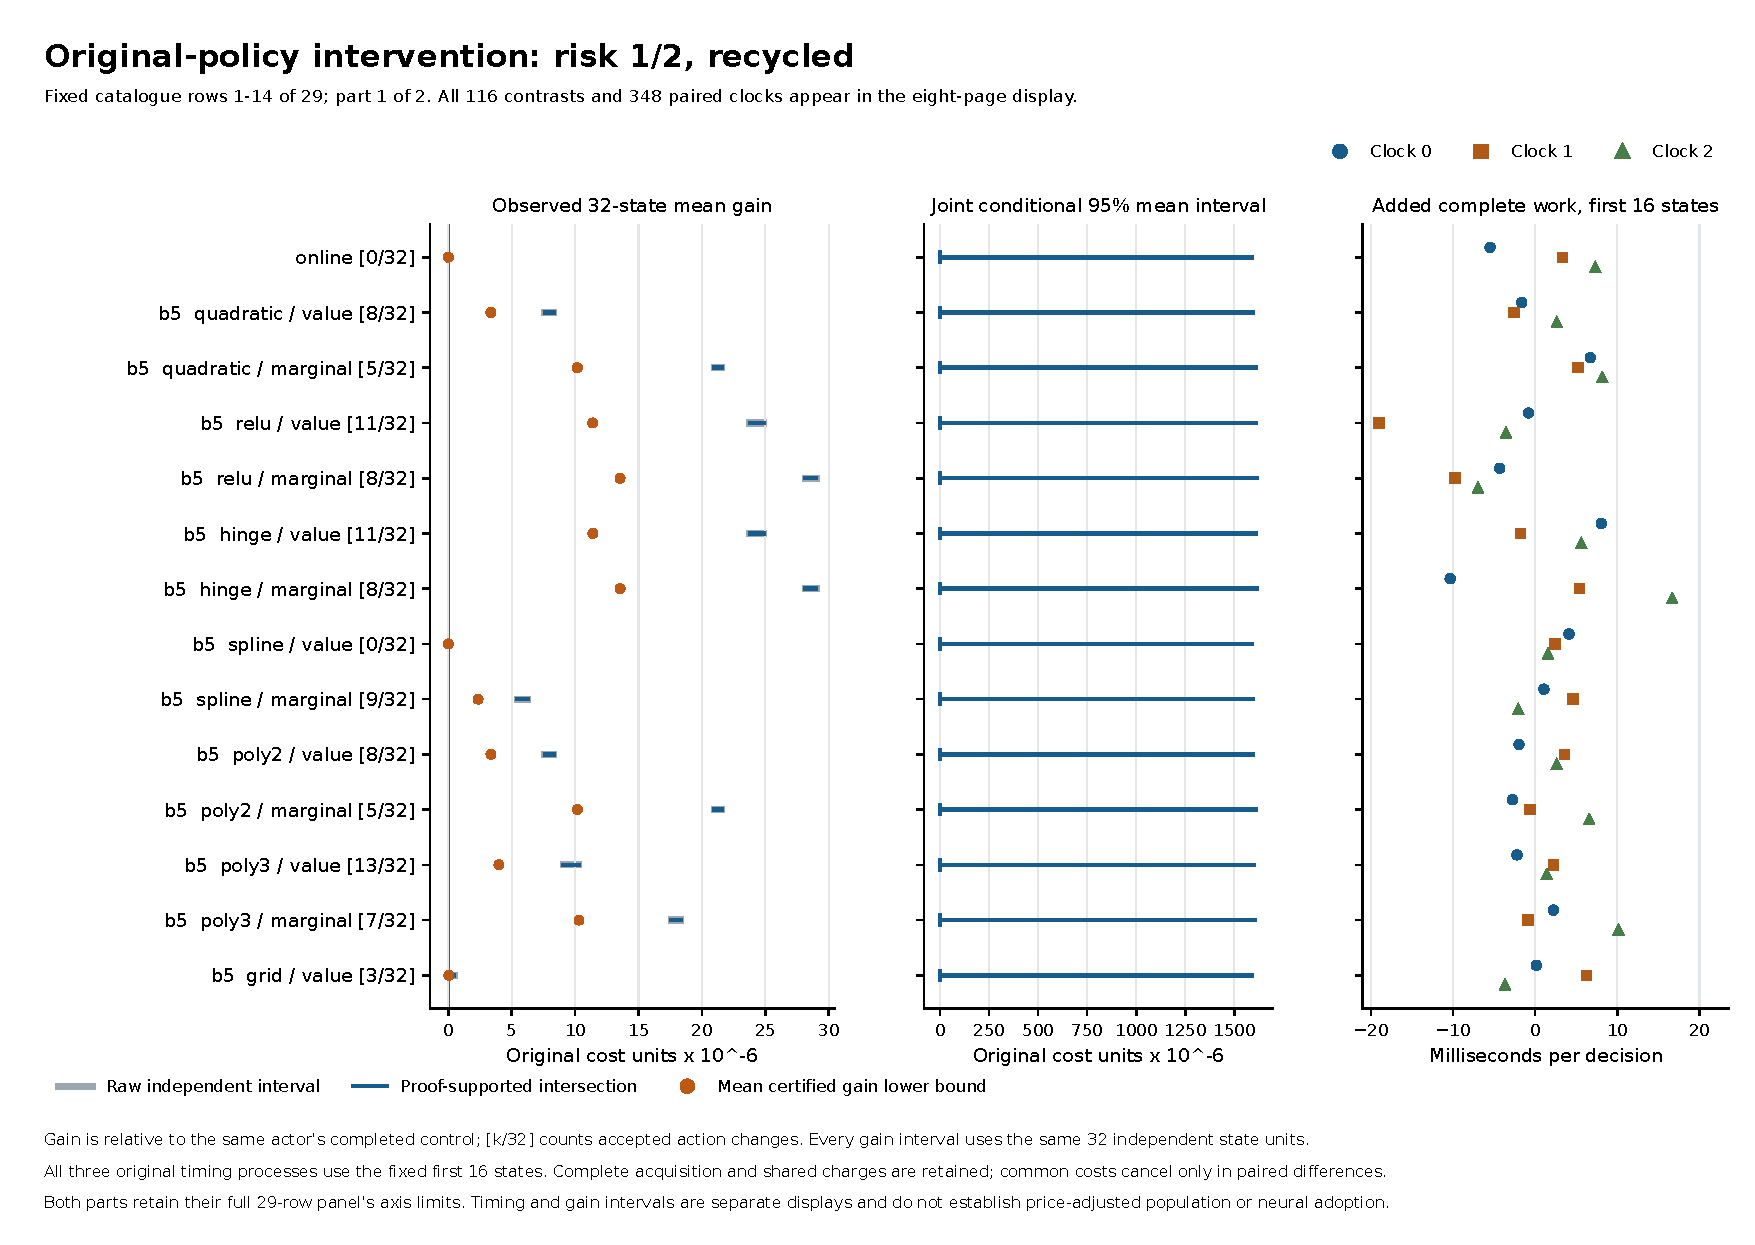
\includepdf[pages=-,fitpaper=true,pagecommand={\thispagestyle{empty}}]{figures122/runtime03-display/complete_catalogue_display122.pdf}
\clearpage
\endgroup
